\section{MakeCode: Design and Implementation}
\label{sec:makecode}

\begin{figure}[t]
    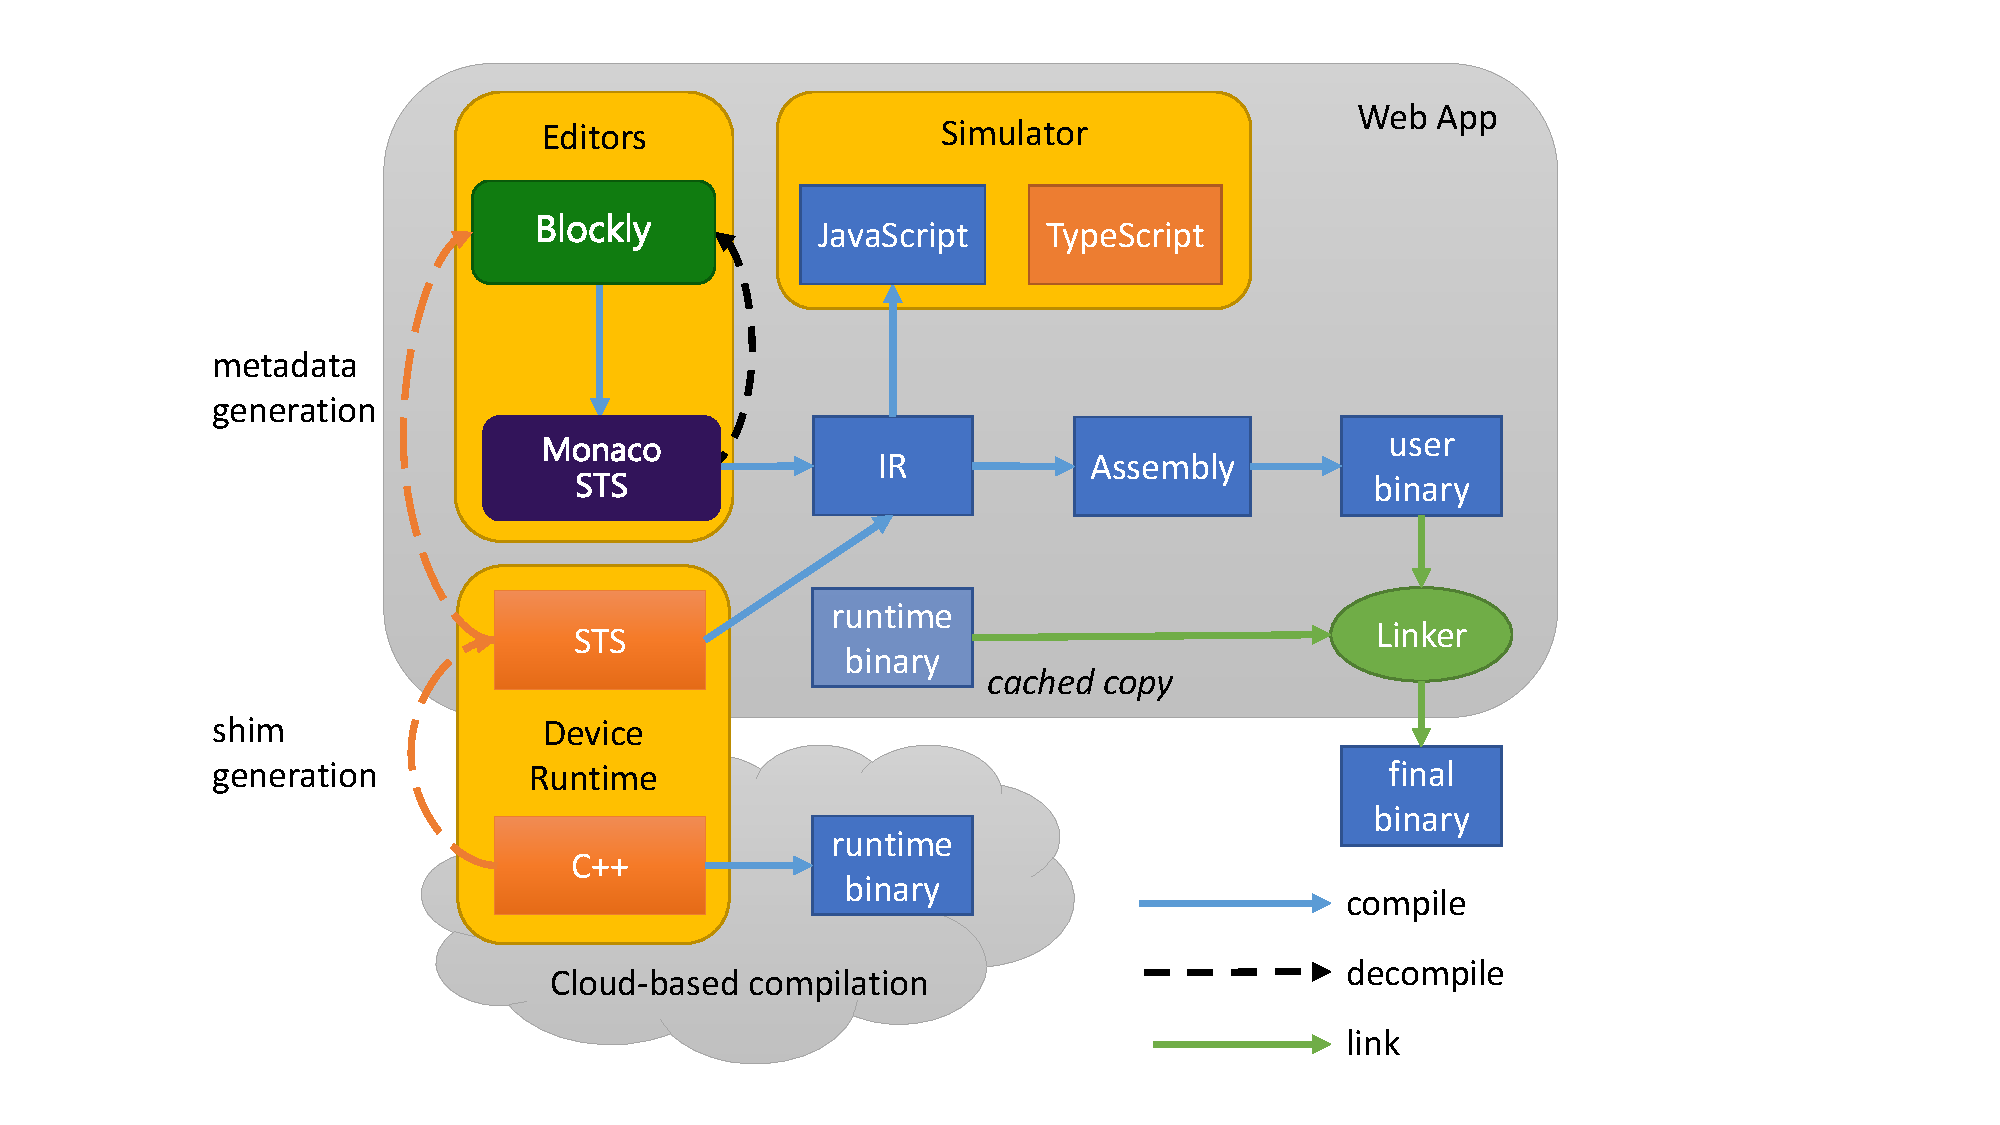
\includegraphics[width=4.5in]{diagrams.pdf}
\caption{\label{fig:makecode}MakeCode Architecture}
\end{figure}

The MakeCode web app encapsulates all the components needed to deliver a programming experience 
for microcontroller-based devices, free of the need for a C++ compiler for the compilation of user 
code, as shown in Figure~\ref{fig:makecode}. 
The web app is written in TypeScript. The web app also incorporates the TypeScript compiler and 
language service (www.typescriptlang.org) which are used in several ways, as detailed below. 
The remaining subsections describe the parts of Figure~\ref{fig:makecode}.

\subsection{Device Runtime and Shim Generation}

A MakeCode target is defined, in part, by its device runtime, which can be a combination of C++ 
and Static TypeScript (STS) code. The C++ runtime for the target microcontroller is precompiled 
and stored in the cloud. The C++ runtime binary is cached in the HTML5 application cache (with 
other assets) so that the web app can function when the browser is offline. Additional runtime
components may be authored in STS, which allows the device runtime to be updated without the need
for any C++ programming, and permits components of the device runtime to be shared by both the device
and simulator runtimes.  We will describe later how elements of the C++ runtime are exposed to STS
(via automated shim generation). The ability to author the device runtime in both STS and C++ is
a unique aspect of MakeCode's design.

Whether runtime components are authored in C++ or STS, all runtime APIs are exposed as fully-typed
TypeScript definitions (for runtime components written in TypeScript) or declarations (for runtime
components written in C++). A full-typed runtime improves the end-user experience by making it easier
to discover APIs; it also enables the type inference provided by the TypeScript compiler to infer types
for (unannotated) user code.

MakeCode supports a simple foreign function interface from TypeScript to C++ based on namespaces,
enumerations, functions, and basic type mappings. MakeCode uses top-level namespaces (in both C++ and
TypeScript) to organize sets of related functions.  Preceding a C++ namespace, enumeration, or function
with \emph{//\%} indicates that MakeCode should map the C++ construct to TypeScript.
Within the \emph{//\%} comment, attributes are used to define the visual appearance for that
language construct, such as for the led namespace in the micro:bit target:

\begin{lstlisting}
//% color=#5C2D91 weight=97 icon="\uf205"
namespace led { 
...
\end{lstlisting}

Here is the C++ file defining the micro:bit's led namespace and its functions:
\begin{center}
\url{https://github.com/Microsoft/pxt-microbit/blob/master/libs/core/led.cpp}
\end{center}

Mapping of functions and enumerations between C++ and TypeScript is straightforward. 
Here's an example of the C++ function plot in the led namespace that wraps a more
complex function call of the underlying device runtime to set/plot an LED in the micro:bit display:

\begin{lstlisting}
//% blockId=device_plot block="plot|x %x|y %y"
//% x.min=0 x.max=4 y.min=0 y.max=4
void plot(int x, int y) {
    uBit.display.image.setPixelValue(x, y, 1);
}
\end{lstlisting}

We'll describe the attribute definitions in the \emph{//\%} comment in the next section. 
MakeCode uses a  TypeScript declaration file to describe the TypeScript elements corresponding
to C++ namespaces, enumerations and functions.  We call such files shim files.
Since the C++ plot function is preceded by a \emph{//\%} comment, 
MakeCode adds the following TypeScript declaration to the shim file (shims.d.ts) and copies
over the attribute definitions in the comment. MakeCode also adds an attribute definition mapping
the TypeScript shim to its C++ function (shim=led::plot):

\begin{lstlisting}
//% blockId=device_plot block="plot|x %x|y %y
//% x.min=0 x.max=4 y.min=0 y.max=4 shim=led::plot
function plot(x: number, y: number): void;
\end{lstlisting}

Here is the shim file generated from the annotated C++ sources for the micro:bit device runtime: 
\begin{center}
\url{https://github.com/Microsoft/pxt-microbit/blob/master/libs/core/shims.d.ts}
\end{center}

To support the foreign function interface, MakeCode defines a mapping between C++ and TypeScript types.
Boolean and void have straightforward mappings from C++ to TypeScript (bool → boolean, void → void). 
As JavaScript only supports number, which is a C++ float/double, MakeCode uses TypeScript's support
for type aliases to name the various C++ integer types commonly used for microcontroller programming
(int $\rightarrow$ int32, unsigned $\rightarrow$  uint32, short $\rightarrow$ int16, 
byte $\rightarrow$ uint8, sbyte $\rightarrow$ int8).  This is particularly
useful for saving space on 8-bit architectures such as the AVR. 

MakeCode supports both untagged and tagged integers (described more later).  Under the untagged strategy,
a JavaScript number is interpreted as a C++ int by default, while the tagged strategy allows both
interpretation as integer and double (with an optimization to convert from integer to double, as required).  
MakeCode includes reference counted C++ types for strings (StringData*) and parameterless lambdas (Action).

These C++ types are mapped to the TypeScript types string and ()=>void, respectively.
MakeCode allows a set of C++ functions with the same first parameter (of type Foo) to be
exposed as a TypeScript interface Foo as follows: this set of C++ functions must be grouped
inside a namespace of the name FooMethods.  See, for example, how a C++ buffer abstraction is exposed:

\begin{center}
\url{https://github.com/Microsoft/pxt-microbit/blob/master/libs/core/buffer.cpp}
\end{center}

You can find the resulting TypeScript Buffer interface in the shim file for the micro:bit
(already referenced above). 

\subsection{Block Metadata Generation}

Both C++ and TypeScript APIs can be specially annotated (minimally via 
\emph{//\% block}) so that the MakeCode compiler generates the needed
Blockly metadata to expose an API as a visual block. So, to expose the previously
encountered plot function as a visual block (as well as a TypeScript function), one simply needs:
\begin{lstlisting}
//% block
void plot(int x, int y) { . . . }
\end{lstlisting}

Additional attribute definitions can provide text descriptions for the block, project function
parameters (thus simplifying the API available via Blockly), and describe other visual/functional
characteristics of the block.  MakeCode uses the types of function parameters to select appropriate
Blockly widgets.  For example, an enumeration is represented by a dropdown menu in blocks.
For more information on the block-specific annotations, see 
\url{https://makecode.com/defining-blocks}. 
MakeCode's support for Blockly means that for the common case, the target developer doesn't need
to know anything about the Blockly framework.  For more sophisticated needs, one can directly access
the Blockly framework. 

\subsection{Editors and Code Conversion}

MakeCode uses the Blockly (\url{https://github.com/google/blockly}) and Monaco 
(\url{https://github.com/Microsoft/monaco-editor}) editors to allow the user to code with
visual blocks or TypeScript. The editing experience is parameterized by the full-typed device
runtime, which provides a set of categorized APIs to the end-user, based on namespaces, as
previously described. These APIs are visible in both editors via a toolbox to the immediate
left of the programming area. The Blockly and Monaco toolboxes show the same set of APIs, to
help in transition from coding with blocks to coding with JavaScript. More advanced TypeScript
APIs can be discovered in Monaco via code intellisense.

The Blockly program representation is compiled to Static TypeScript in a syntax-directed manner
(see \url{https://github.com/Microsoft/pxt/tree/master/pxtblocks}). A key issue is the need for
type inference on the Blockly representation, as variables generally are defined and used without
being declared in Blockly. MakeCode uses a simple unification-based type inference to assign a
unique type to each variable.  In the future, we expect to use TypeScript's type inference instead
and eliminate the need for separate type inference over the Blockly representation. 
TypeScript supports programming constructs that are not available in Blockly, such as classes.
Such constructs are converted into grey uneditable blocks in Blockly, with the construct's program
text intact. This means MakeCode always can decompile a TypeScript program to Blockly and then recover
the program text of the grey blocks when converting from Blockly back to TypeScript
 (see \url{https://github.com/Microsoft/pxt/blob/master/pxtcompiler/emitter/decompiler.ts}). 

\subsection{Compilation Pipeline}

MakeCode first invokes the TypeScript language service to perform type inference and type checking on the 
user's program, using the TypeScript declaration files for the device runtime.   It then checks that the
user's program is within the STS subset through additional syntactic and type checks over the adorned
abstract syntax tree (AST) produced by the language service (detailed in Section XYZ).  Assuming all the
above checks pass, MakeCode then performs tree shaking and compilation of the AST of the user code and
device runtime to an intermediate representation (IR) that makes explicit: labelled control flow among a
sequence of instructions with conditional and unconditional jumps; heap cells; field accesses; store operations,
and reference counting.

There are two backends for code generation from the IR. The first backend simply generates JavaScript,
for execution against the simulator runtime.  The other backend generates assembler, parameterized by a
processor description.  Currently supported processors include ARM's Cortex class (Thumb instructions)
and Atmel's Atmega class (AVR instructions). A separate assembler, also parameterized by an instruction
encoder/decoder, generates machine code. Finally, a linker completes the compile chain by resolving
references to the driver runtime in the user's program, producing a binary executable. The compiler chain
can be found at \url{https://github.com/Microsoft/pxt/tree/master/pxtcompiler/emitter} and 
\url{https://github.com/Microsoft/pxt/tree/master/pxtlib/emitter}.

\subsubsection{Asynchronous Functions}

A key part of the compilation process is to allow users to call async functions (identified through
the \emph{//\% async} annotation) as if they were regular (blocking) functions.  This is done by
compiling each function so that it can be suspended (at the return of a call) and later resumed (at the same point). 
The default behavior at a suspension point is to immediately resume execution.  If a call is to an async function then
the default behavior is overridden by the compiler, which suspends execution of the current function. Upon completion
of the async function call, the current function then is resumed.    This feature greatly simplifies the JavaScript-based
programming model which relies on promises to achieve asynchronous execution, breaking up sequential (blocking) code into
a series of event handlers.  The JavaScript-based simulator runtime uses promises to achieve asynchronous execution in a
single-threaded context, but these promises are hidden from the end user.    The CODAL C++ device runtime supports fibers
with the ability to pause, so for compilation to a device, the compiler simply emits a call to pause at a suspension point. 

\subsubsection{Untagged and Tagged Strategies}

The MakeCode compiler supports the Static TypeScript language subset described in Section X, with two compilation
strategies: untagged and tagged. 
\emph{TODO}
Untagged compilation strategy
No support for doubles. 32-bit integers (signed only). Use static type system to distinguish between integers and references.
No runtime support.  Not fully compatible with JavaScript semantics. Null = Undefined = 0 = default integer value.  Support for
different integer sizes using type aliases (this is used for AVR). 
Tagged compilation strategy
In the tagged strategy, numbers are either tagged 31-bit signed integers, or if they do not fit, boxed doubles. Code generation
to check tag bit. Special constants like false, null and undefined are given special values and can be distinguished. Fully
compatible with JavaScript semantics (number, null, undefined).   Can accommodate a richer type system. 

\subsection{Simulator}

A MakeCode target can provide an alternate TypeScript implementation for each API in the device runtime, for use in the device
simulator. As this code runs in the web browser (not on the actual device) and manipulates the DOM, the developer is free to
use all of TypeScript/JavaScript's features. (As an aside, MakeCode also support ``simulator-only'' targets that have no 
associated device; in these cases, the ``device runtime'' is defined solely by the simulator APIs.) 
The simulator allows the user to experience the basic functions of the device in the browser and to test their code
before deploying it to the actual device. The simulator has proxy widgets for sensors such as accelerometer (mouse motion),
temperature and light, allowing the user to control the sensor's value.  The simulator only provides basic functionality
and is far from a complete device emulation.   For example, it is not possible for the user to simultaneously modify two
inputs to the simulated device, while it is possible with the actual device (i.e., shaking it to change the accelerometer
reading while pushing one of the device's buttons).

MakeCode provides various components to make device-based simulators easier to build: board, parts, wiring, etc.

\subsection{Packages and Custom Editors}

Packages are MakeCode's dynamic/static library mechanism for extending a target (by adding new code/data to the device
and simulator runtimes, as well as accompanying documentation). The following package extends the micro:bit target so
that the micro:bit can drive a NeoPixel strip of RGB LEDs: \url{https://github.com/Microsoft/pxt-neopixel}. To see how this
package is surfaced to the end-user, visit \url{http://makecode.microbit.org/} and select the ``Add Package'' option from the
gear menu; you will see the package ``neopixel'' listed in the available options. If you click on it, a new block category
named ``Neopixel'' will be added to the editor. In this scenario, PXT dynamically loads the (white listed) neopixel 
package directly from GitHub, compiles it and incorporates it into the web app. Packages also can be bundled with a web
app (the analog of static linking).  

Hardware partners already have started to create MakeCode packages for the micro:bit.
Seeed Studio (\url{https://www.seeedstudio.com/}) has created packages to add its Grove components to a micro:bit.
Grove components are accessed via the I2C serial protocol, supported by the micro:bit device runtime.
All micro:bit packages for the Grove components are authored in Static TypeScript (gesture, ultrasonic-ranger,
4-digital-display, two-led-matrix). These packages can be found under GitHub user ``Tinkertanker'', prefixed with
``pxt-''. Sparkfun has created MakeCode packages for its micro:bit shields (GitHub user ``sparkfun'').

% https://github.com/Tinkertanker/pxt-ssd1306-microbit
% https://github.com/Tinkertanker/pxt-ir-microbit 
% https://github.com/Tinkertanker/pxt-ky040-microbit
% https://github.com/Tinkertanker/pxt-ds1307-microbit
% Sparkfun
% •	https://github.com/sparkfun/pxt-weather-bit
% •	https://github.com/sparkfun/pxt-moto-bit 
% •	https://github.com/sparkfun/pxt-gamer-bit 
% Common packages
% •	https://github.com/Microsoft/pxt-common-packages
% •	Structure:
% o	Libs/package/
% [talk about C++] Various examples.
% [more about customer editor associated with a package]
